\chapter{Варяги}
%\corner{64}
\vepsianrose
\fancyhead[LE]{\fancyplain{}{\bfseries \parttitle}}
\fancyhead[RO]{\fancyplain{}{\bfseries \rightmark}}

\diagdash Так, отряд, подъём!!!\mdash громогласно огласил Адмирал, поднимаясь с кровати.

\diagdash Шурик, имей совесть, дай поспать!

\diagdash Вперёд! Нас ждут великие дела! Сегодня по плану осмотр крепости и ещё 400 километров до Карелии!

\diagdash Кто сёдня дежурный по завтраку, а?

Команда тяжеловато выползла из номера и спустилась на кухоньку завтракать\mdash гостиница была и впрямь скромная, но на кухне имелась посуда, техника, короче всё что нужно. Ребята быстренько перекусили и двинули в~сторону крепости пешком\mdash идти было около километра.

\diagdash А давай вон туда?\mdash Серёга показал на ответвление к реке через парк, хотя к крепости было прямо.

\diagdash Нафига? Нам прямо$\ldots$\mdash изнывая от жары отбивался Адмирал.

\diagdash Забей, пойдём глянем реку! Поздороваемся, так сказать, с водой!\mdash настаивал Серёга.

И они прошли сквозь парк вдоль стены монастыря к~реке. Вид на реку Волхов был, надо признать, шикарен. Берег внизу утопал в растительности\mdash непролазные заросли кустов и прибрежной травы устилали весь подъём от~воды. Степ\'{е}нные в\'{о}ды ползли, как и сотни лет назад, вперёд к~Ладожскому озеру.

\diagdash Давай вдоль монастыря срежем?\mdash не унимался Серёга.

\diagdash Ой не нравится мне это.\mdash попробовал отбиться Адмирал.

\diagdash Давай, погнали! Не обратно же идти.

Ребята пошли по тропинке вдоль стены монастыря, обращённой к~реке. Народу, естественно, было никого\mdash они шли по едва хоженой тропке между кирпичной кладкой монастырских стен и берегом реки, утопающем в буйной растительности. Примерно посредине той стены им встретились старые заколоченные монастырские ворота. Вероятно, тут когда\sdash то был причал. Однако сейчас выхода к~воде не было\mdash сплошные заросли. 

\diagdash Вообще\sdash то это Староладожский Успенский женский монастырь, сюда Евдокию Лопухину царь Пётр I сослал, когда она ему осточертела, видать.\mdash сказал Шурик.

\diagdash О как просто\sdash то!\mdash оживился народ.

\diagdash Конечно просто, когда ты\mdash царь. А между прочим, это была последняя русская жена монарха, потом всё по~известному органу пошло\mdash Екатерина I, его вторая жена, вообще то ли латышка, то ли немка, то ли чёрт знает кто\mdash ни кровей, ни черта, но грудь там знатная, конечно если художники не врут. Потом цари на наших больше не~женились. Вот когда у~нас всё~в~истории пошло не~так! Со времён смуты, XVI\thinspace\nobreakdash---\thinspace XVII век, ха! Пойдём быстрее, а? Жарко$\ldots$\mdash Шурику  хотелось быстрее в крепость.

\diagdash Шу-у-урик, это ты всё со школьной истории помнишь?\mdash спросил Серёга.

\diagdash Ага, с утра в Интернете прочитал$\ldots$

\vspace{1.0cm}
$\ldots$Когда они прошли больше половины стены, впереди показалась крепость. Вскоре команда миновала узкую тропинку, идущую вдоль монастыря, и~вышла к~скверу, в~торце которого обнаружился памятник Рюрику и~Вещему~Олегу. 

\diagdash Монументально!\mdash Замполит обошёл кругом изваяние.

\diagdash Ха! А то! Цветмета сколько, натурально!!!

Дальше друзья спустились к смотровой площадке, с~которой открывался замечательный вид на Стрелочную башню крепости, названную так, собственно, потому что она стоит на самом мысу, на стрелке, у впадения реки Ладожки в~Волхов\mdash просто идеальнейшее место для оборонительного сооружения, c двух сторон естественное препятствие для атакующих\mdash река.

Подкатил туристический автобус, из которого высыпалась группа с экскурсоводом, тут же начавшим свою нудятину:

\diagdash Здесь вы можете видеть$\ldots$

Ребята, нафоткавшись на фоне башни, поспешили из~сквера к мосту, чтобы уже перейти к подножию самой крепости. Повсюду было прилично народу\mdash люди приезжали на своих авто и экскурсионных автобусах.

Если вчера крепость, когда они проезжали мимо неё, казалась какой\sdash то маленькой, как игрушка почти, то~сейчас, стоя у подножия её стен, ребята воочию могли убедиться, что это не так. Высоченные стены и грозные башни, жалко, конечно, что восстановленные, производили самое суровое впечатление. Шурик вдруг на~минуту подумал о~том, как тяжело, если не невозможно, было в~IX\thinspace\nobreakdash---\thinspace X~веке штурмовать такое сооружение и какое угнетающее впечатление производило всё это на атакующих.

Восстановление крепости было начато ещё в советское время, но тогда успели сделать только две башни. Сейчас же, к 900\sdash летию Старой Ладоги, восстановили почти всё, кроме крепостной стены, обращённой к реке Волхов, и земляного городища, располагавшегося уже за пределами крепости к~югу. Современный вид крепости со стороны дороги и вовсе шикарен\mdash наверное почти не уступает историческому. 

\diagdash Нет, не скифы, не азиаты мы! Мы\mdash варяги, едрёна вошь!\mdash распалялся Шурик, воображение которого разыгралось не на шутку от увиденного.

\diagdash Пошли, варяг, блин, нашёлся!\mdash ребята прошли сквозь Воротную башню.

{
	%\begin{wrapfigure}{l}{0.7\textwidth}
	\begin{figure}[h]
		\centering
		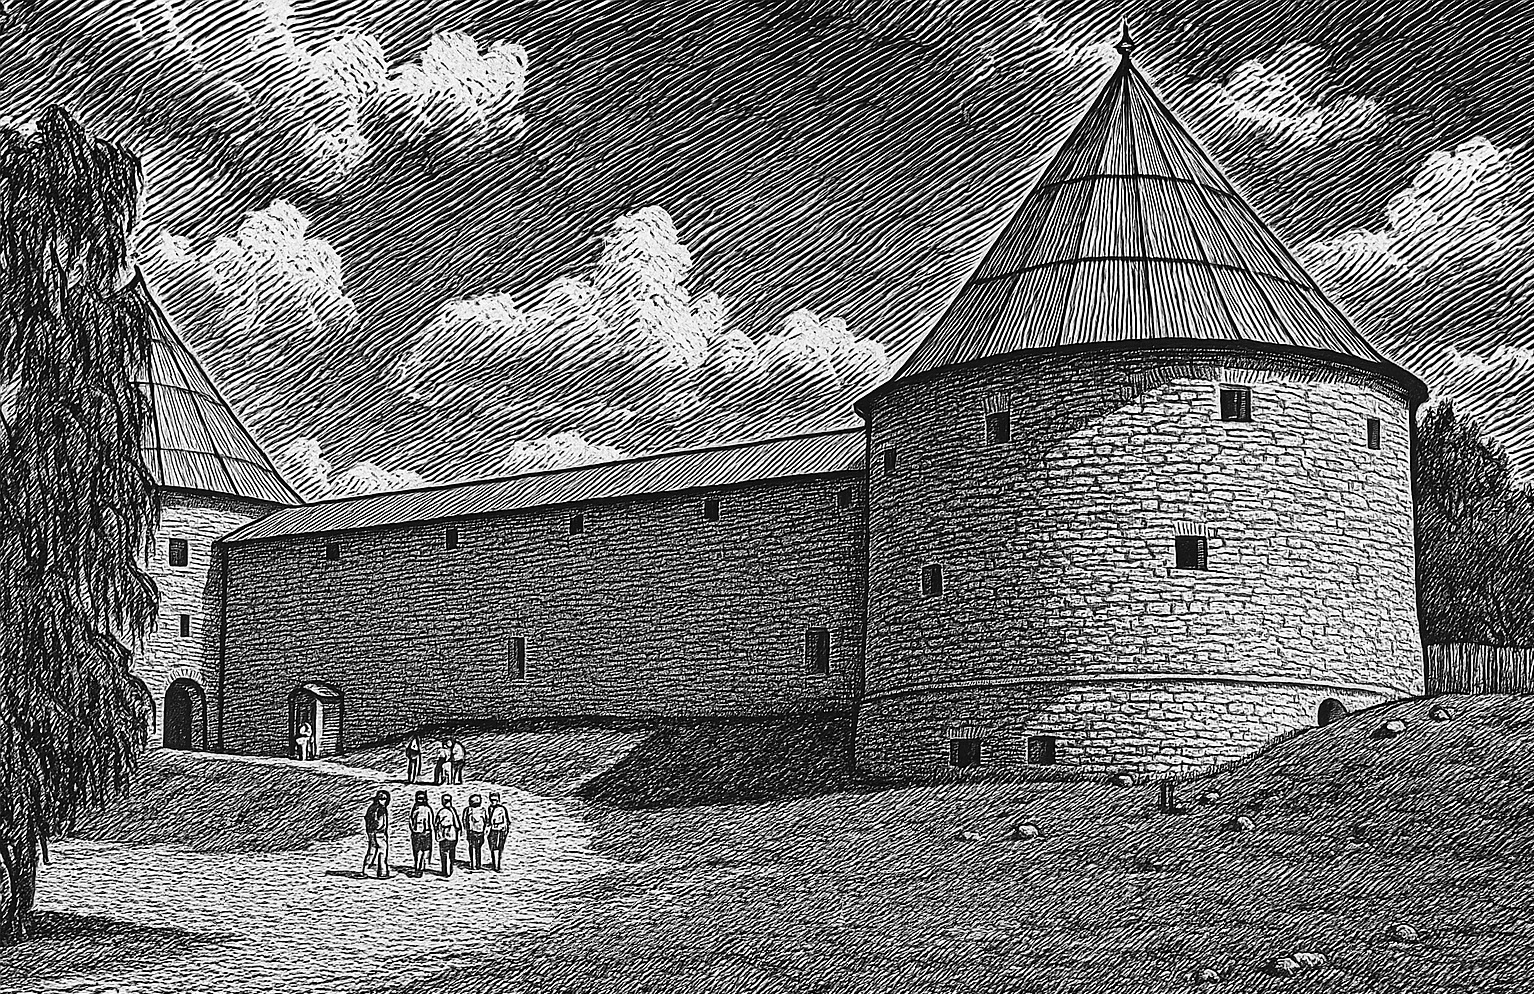
\includegraphics[width=1.0\textwidth]{07_ladoga}
		\caption{\small\textit{...нет, не скифы, не азиаты мы...}}
	\end{figure}
	%\end{wrapfigure}
}

В крепости была устроена отличная экспозиция внутри башен и команда поспешила со всем этим ознакомиться. В Стрелочной башне был представлен макет крепости, различные археологические находки, обнаруженные тут же при~раскопках. Над оснащением музея хорошо поработали\mdash тут были разные интерактивные экраны для детей, множество экспонатов, доспехи, оружие и~прочее\sdash прочее\sdash прочее. На стенах внутри Раскатной башни висели плакаты с~восстановленным историческим обликом крепости. Ребята сходили и~на~Климентовскую башню, в~которой также была выставка, для чего надо было подняться на толстенную крепостную стену. Шурик про себя отметил некую горечь, что почти всё вокруг\mdash восстановленное, поскольку он видел раньше цветные ретро\sdash фотографии крепости, сделанные в начале XX~века по технологии совмещения трёх фотографий, снятых через светофильтры разного цвета\cite{ПрокудинГорский}\mdash там всё лежало в руинах.

Считается, что Староладожская крепость была основана в VIII веке выходцами с острова Готланд~\cite{ЛебедевЛадога}. Закрывая путь с севера на~Русские Земли, она многократно подвергалась нападениям скандинавов, которые не раз разрушали её, но она каждый раз возрождалась\mdash уж больно хорошим и стратегически выгодным было это место на стрелке у впадения р.\thinspace Ладожки в Волхов.

Ребята посетили все доступные места, облазили стены и вышли на самый верх Раскатной башни, где была устроена смотровая площадка. Шурик сделал панорамный снимок этой красоты и поспешил за командой, которая уже собралась во внутреннем дворике крепости, около церкви.

Осмотрев в крепости, пожалуй, всё, что можно было осмотреть, команда двинулась на выход\mdash время шло к~обеду. Осмотр отнял прилично времени, но его было не~жаль\mdash это действительно того стоило. 

По дороге обратно Шурику стало маленько дурно\mdash яркое солнце напекло голову, жара вокруг стояла приличная:

\diagdash Кирь, а ты боялся холодов!

\diagdash Погоди, до Карелии ещё не добрались!

Команда вновь разделилась\mdash Серёга и Руслан отправились обедать в местный ресторанчик, а Киря, Шурик и Паша решили скорее двинуть дальше и отобедать где\sdash нибудь по пути. В машине их ждал спасительный кондиционер.

\diagdash Так! Тащ Замполит!\mdash Шурик поскорее завёл машину и врубил кондиционер на максимум, умирая от~жары.

\diagdash Я!

\diagdash Поищи где отобедать по пути?%, чёт голодно.

\diagdash Ну это уже в Сясьстрое наверно, тащ Адмирал.

\diagdash Это далеко?

\diagdash Момент$\ldots$\mdash Замполит копался в навигаторе.\mdash Через 25 минут будем на месте!

\diagdash Там есть что\sdash нибудь приличное?\mdash засомневался сзади Паша.

\diagdash Кафе <<Встреча>>,\mdash огласил Киря,\mdash отзывы хорошие$\ldots$

$\ldots$Друзья отобедали в очень приличном кафе самообслуживания и двинули дальше, созвонившись с~остальной частью команды\mdash те только выползли из~трапезной в Старой Ладоге. 

Вскоре, в Лодейном Поле, друзья пересекли реку Свирь по огромному разводному мосту, весь центральный пролёт которого может подниматься горизонтально вверх для~пропуска высоких судов. Мост их впечатлил\mdash махина что надо! Дальше начались уже типично карельские пейзажи\mdash хвойные леса с мшаниками, узкая дорога. До Петрозаводска было, казалось, рукой подать, но дорога выматывала монотонностью. Ребята проехали арку над дорогой, где было написано <<Республика Карелия приветствует Вас!>>, то~есть официально пересекли границу Карелии. Дорога шла как масло, но однополосная. Вскоре Шурик стал ну~просто засыпать за рулём, один раз даже наехал правыми колёсами на вибро\sdash акустические <<пробудители>>:

\diagdash Э\sdash э\sdash э! ШУРИК!!! Не спать!\mdash всполошился Киря.

\diagdash Не сплю, не сплю, всё норм!\mdash сам ошалевая от звука и вибрации пробудителей очнулся Шурик. Только сейчас он заметил, что уже давно, с полчаса точно, вдоль правого края дороги часто шли прямоугольные выемки\mdash он ещё подумал зачем они нужны. Теперь на собственной шкуре понял зачем. <<Хорошо не на встречку>>,\mdash подумалось Шурику.

\diagdash Хочешь, я поведу?\mdash спросил Паша, и они сделали остановку на 5 минут перекурить и поменяться местами. После Шурик устроился на переднем пассажирском и уже спустя пару минут его просто вырубило\mdash ему всё\sdash таки напекло солнышко, пока друзья ходили по Староладожской крепости$\ldots$

\vspace{0.5cm}

$\ldots$Очнулся Шурик уже за Петрозаводском. Паша сел на хвост какому\sdash то дальнобою и ехал неспеша. Он~аккуратно вёл, Шурик даже выспался немного.

\diagdash Вот это меня рубануло, пацаны\mdash Шурик тёр усталые глаза.

\diagdash Ну да, скоро Кондопога.\mdash сонно отозвался Киря.

\diagdash А давайте на Кивач заедем?\mdash предложил чуть оживший Шурик.\mdash Когда ещё тут будем\sdash то?

\diagdash Это по пути? Там водопад и всё?

\diagdash Агась. Вообще\sdash то это один из самых больших водопадов Карелии. Я хотел потом, на выброске, туда зарулить, но что\sdash то мне подсказывает, что лучше сейчас.\mdash заключил Шурик.

\diagdash Потом уже будет домой хотеться, так что давайте реально щас.\mdash подал сзади голос Киря.

\diagdash А поехали! Напиши Серёге, чтоб тоже заезжал.\mdash согласился Паша.

Вскоре ребята свернули у указателя <<Кивач>> и~запарковались перед въездом на территорию. Совсем скоро подкатила вторая часть команды, и они вместе пошли в~заповедник, приобретя билеты.

Вечерело, было около половины восьмого, все лавочки с сувенирами и прочим были закрыты. Путешественники вышли к водопаду, рёв которого начинался уже за сотню метров. Кивач был шикарен, кто бы что ни говорил! Несметные толщи воды низвергались с десятиметровой высоты, протекая между скал и разбиваясь внизу на~миллиарды миллионов белоснежных брызг, окатывающих синеющие скалы. Рёв вблизи был просто оглушающим\mdash чувствовалась мощь природной стихии. 

%\begin{wrapfigure}[21]{r}{0.5\textwidth}
%	\centering
%	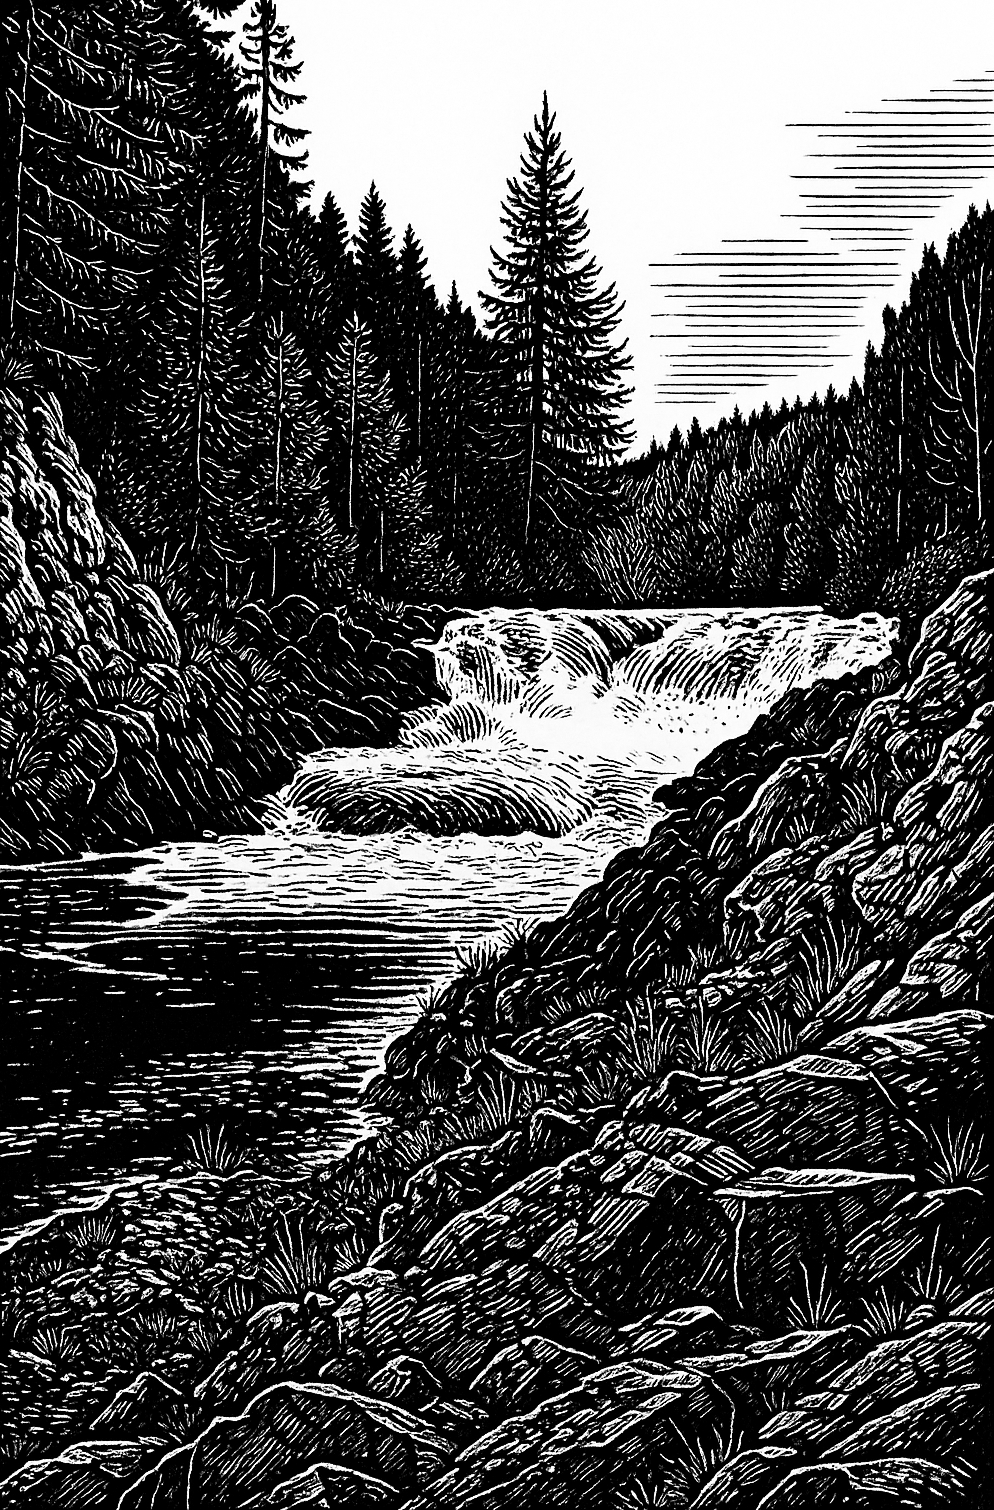
\includegraphics[width=0.5\textwidth]{5_2_new2}
%	\caption{\small\textit{...жемчужина Карелии...}}
%\end{wrapfigure}
%Смотровая площадка располагалась после 4-й ступени водопада, самой высокой, а~немного выше был виден предыдущий каскад с~двумя чуть меньшими водопадиками. Друзья забрались в~самый дальний край тропинки на~гору, где была установлена лавочка и~открывался чудесный вид вниз на~долину. Присели на лавочку передохнуть и~подождать Серёгу с~Русланом.

\noindent
\begin{minipage}{0.45\textwidth}
	\setlength{\parindent}{1.0cm}  % Восстановление отступа абзаца
	
	\indent Смотровая площадка располагалась после 4-й ступени водопада, самой высокой, а~немного выше был виден предыдущий каскад с~двумя чуть меньшими водопадиками. Друзья забрались в~самый дальний край тропинки на~гору, где была установлена лавочка и~открывался чудесный вид вниз на~долину. Присели на лавочку передохнуть и~подождать Серёгу с~Русланом.
	
	\indent Кивач\mdash жемчужина Карелии. Заповедник был \makebox[\linewidth][s]{\noindent создан в~30\sdash ые годы XX\hspace{0.25em}в.}
\end{minipage}\hfill
\begin{minipage}{0.5\textwidth}
	\centering
	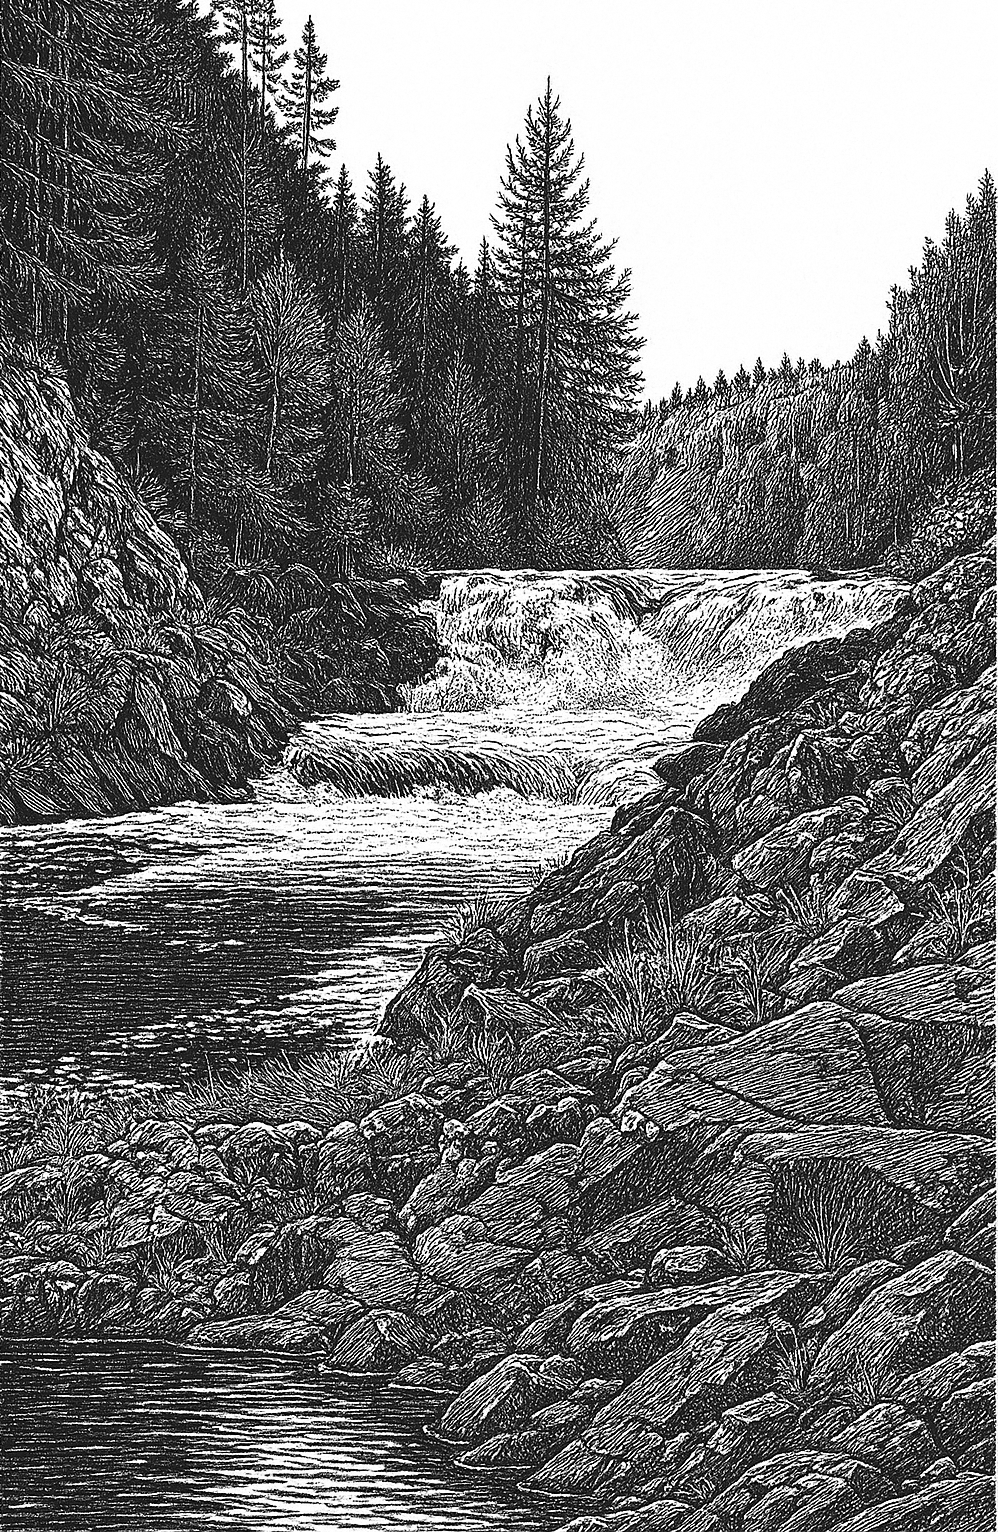
\includegraphics[width=\linewidth]{08_kivach}
	
	{\small\textit{...жемчужина Карелии...}}
\end{minipage}

%Кивач\mdash жемчужина Карелии. Заповедник был создан в~30\sdash ые годы XX века и с тех пор стал местом 
\newpage
\noindent и~с~тех~пор стал местом притяжения туристов и~отдыхающих. Природа~в~заповеднике по\sdash северному красива\mdash здешними видами восторгался ещё~Прокудин\sdash Горский, запечатлевший водопад Кивач на~первые в~мире цветные фотографии этого места, вошедшие позже в альбом <<Мурманская железная дорога>>. Но~когда в~50\sdash х годах XX\hspace{0.25em}в. была построена Пальозёрская ГЭС, уровень воды изменился и~былые виды у~водопада исчезли. Шурик пытался по~ретро\sdash фото\cite{ПрокудинГорский} опознать местность, оказавшись у~водопада, но у~него не~получилось. В~частности, характерной беседки с~ретро\sdash фото он не нашёл.

Отдохнув на лавочке, друзья пошатались по дендрарию, посетили памятник советским воинам, павшим во время боёв в~Карелии в~Великой Отечественной Войне, и пошли, не~торопясь, назад. Времени уже было к закрытию заповедника, дневная жара наконец\sdash то спала, ребята потихоньку шли на выход. Шурик всё ещё ощущал последствия полуденного теплового удара и~ему было нехорошо, так что плёлся он позади всех, не~забывая фотографировать окрестности. 

Друзья вернулись к~машинам и~резво рванули преодолеть последнюю часть пути до~Гирваса, в~который они и прибыли в половину десятого~вечера, закупившись в~местном магазинчике на~вечер.

Они проехали через почти весь посёлок в район Пальозёрской ГЭС и запарковались у маленькой гостиницы. Расположились, перетаскали вещи. Пашка начал накачиваться пенным уже таская шмот, остальные присоединились почти сразу же\mdash усталость так и валила всех с ног. Надо было ещё перепаковать снарягу, но сначала все решили перевести немного дух\mdash длинная дорога давала о себе знать. Команда разбрелась по просторному номеру, состоявшему из большой комнаты, террасы и санузла. 

%\newpage
Шурик, пока все приходили в себя после дороги, занял душевую и~освежился\mdash водичка была еле тёплой и мощно взбодрила его так, что он даже замёрз:

\diagdash Бр-р-р, пацаны! Водичка огонь! Давай, кто следующий?\mdash растираясь полотенцем, вышел из душа Адмирал. Всё, городская одежда снята, тело умыто карельской водой\mdash Шурик почувствовал очередной прилив энергии преображения из вчерашнего Городского Жителя в~Адмирала. Окончательно они преобразятся только встав на воду и найдя первую стоянку$\ldots$

\diagdash Совсем огонь?\mdash поинтересовался Киря, тоже собиравшийся освежиться.

\diagdash Ну потеплее, чем завтра в реке, ы\sdash ы\sdash ы!!!\mdash заржал Адмирал, доставая, чтобы утеплиться, из вещмешка цветастое перуанское шерстяное пончо.

\diagdash Ого, пацаны, Шурик а-ля Клинт Иствуд!\mdash команда заценила прикид.

\diagdash А то! Перефразируя его знаменитую фразу: все сплавщики делятся на два типа\mdash на Адмирала и на тех, кто перепаковывает вещи, ы\sdash ы\sdash ы!\mdash выделывался Шурик.

\diagdash Ща перепакуем, всё будет в наилучшем виде, не~очкуйте!\mdash Замполит сновал по комнате с пивной банкой в~руке, умудряясь при этом перетаскивать мешки с провизией и снаряжением.

Адмирала как осенило:

\diagdash Замполит!!! Знамя полка!

{
	\setlength{\belowcaptionskip}{-10mm}
	%\begin{wrapfigure}{l}{0.7\textwidth}
	\begin{figure}[h]
		\centering
		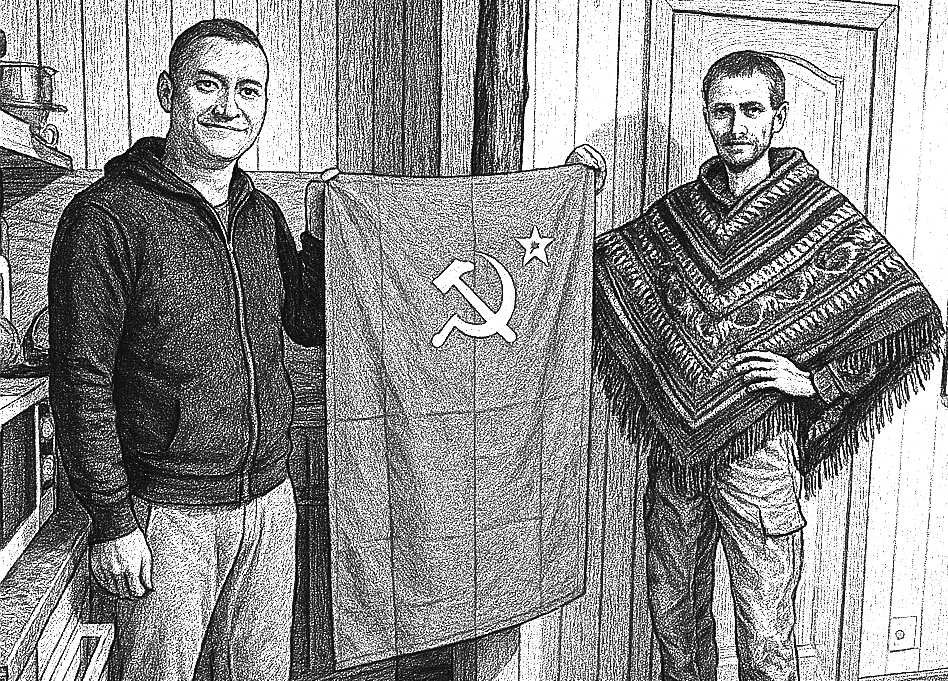
\includegraphics[width=1.0\textwidth]{09_2_ussr}
		\caption{\small\textit{...молоткасто-серпастое...}}
	\end{figure}
	%\end{wrapfigure}
}

Он то ли по привычке, то ли традиции со времён сплава по Чагодоще брал с~собой флаг СССР. Достав и~расправив молоткасто\sdash серпастое ало\sdash красное полотнище, они с Замполитом заорали что есть мочи, прихлебнув пенного:

%\newpage
\vspace{0.2cm}
\noindent\textit{%
	\hspace*{1.2cm}Но на фуражке на моей\mdash серп и молот и звезда,\\
	\hspace*{1.2cm}Как это трогательно\mdash серп и молот и звезда,\\
	\hspace*{1.2cm}Лихой фонарь ожидания мотается\\
	\hspace*{1.2cm}И всё идёт по плану$\ldots$\\
	\hspace*{1.2cm}\large{ВСЁ ИДЁТ ПО ПЛАНУ!}\\
	\hspace*{1.2cm}\Large{ВСЁ ИДЁТ ПО ПЛАНУ!!!}\\
	\hspace*{1.2cm}\LARGE{ВСЁ ПО ПЛА-А-АНУ!!!!!}
}

\vspace{0.2cm}
%\newpage
\diagdash Панки хой!!! Хэви м\'{е}тал форева!!! У\sdash у\sdash х\sdash у\sdash х\sdash у!!!\mdash орали они, пританцовывая$\ldots$

\vspace{0.5cm}
$\ldots$Всё шло своим чередом\mdash народ по очереди стал освежаться в д\'{у}ше. Сейчас оттуда доносились восторженные возгласы Замполита по поводу температуры воды. Серёга разлёгся на кровати, Руслан пока перекусывал. Паша решил перепаковать герму и вывалил все вещи из~неё на свою кровать на терраске. Адмирал же, укутавшись в~пончо, чуть передохнул и согрелся. Надо было собраться с~мыслями, всё доделать и лечь спать. Киря, тем временем, вынырнул из~душевой:

\diagdash Ж-ж-жесть! 

\diagdash С лёгким паром, ы-ы-ы!

Следующий пошёл закаляться в душ, а Киря переоделся и распотрошил свои гермы и сумку. Адмирал вспомнил про сухофрукты, спиральки от комаров и прочее, что должен был купить Замполит:

\diagdash Тащ Замполит! Давай сюды сухофрукты, орехи, энергетические батончики\mdash перепакуем это всё в вещмешки как надо!\mdash вдруг очнувшись, стал командовать Адмирал. Пенное как будто не усыпило его, а придало импульс дожить этот чертовски длинный день. 

\diagdash Лови!!!\mdash отозвался тот и швырнул пакеты. Адмирал поймал и уложил орехи c сухофруктами в видавшие виды и выцветшие от~времени вещмешки. Питательные батончики спортивного питания решили паковать как есть\mdash в~картонных коробочках, чтобы те не помялись.

\diagdash Адмирал! Ещё мой протеин!\mdash гулко выпалил Замполит, разбирая свой шмот.

\diagdash Ты издеваешься?!\mdash отозвался тот.\mdash Качок хренов! Ладно раньше надо было, а щас\sdash то что? Женился ж уже?! Сейчас\sdash то нахрена?\mdash 5\sdash литровая банка со спортивным питанием никуда не влезала, Замполит в итоге решил поставить её в свою красную герму.

\diagdash Как нахрена? Жену молодую впечатлять, ну~чё~ты!\mdash хором отозвались Серёга и Руслан и все дружно подогрето заржали.

\diagdash Ы!\mdash поднялся Паша.\mdash Там и компоты есть в~мешках, сто процентов! Потроши мешки!!!\mdash не унимался рыбак и носовой гребец.\mdash Консервов понабрали, а~бензопилу мою не взяли, ироды!!! У\sdash у\sdash у!!!\mdash и, нетрезво шатаясь, чуть не упав в~дверях, потопал в душ.

%\newpage
Народ, казалось, одновременно был занят перепаковкой вещей, ужином, пенным, помывкой в~д\'{у}ше. Когда все приготовления были окончены, а пенное выпито, народ стал укладываться. Адмирал, забив себе кровать в~уголочке, лёг и, достав из~малой гермы свой командирский планшет с бумажной заламинированной картой похода и~судовым журналом, стал делать путевые заметки\mdash расписал сегодняшний и~вчерашний день, поведал о планах на~завтра, зафиксировал время по своим китайским ролексам и, напрочь окончательно устав, провалился в такой глубокий и тёмный молодецкий сон, какой только может быть у~человека, который завтра должен будет возглавить эскадру. Спать оставалось часов пять.

\begin{center}
	\psvectorian[scale=0.4]{88} % Красивый вензелёк :)
\end{center}

 






